\section{Random Variables and Their Distributions}

In probability theory, the concept of a random variable provides a powerful way to describe quantities that can change due to random processes. As highlighted in the gambler’s ruin problem, instead of cumbersome notation like \( A_{jk} \) for gambler A's wealth after \( k \) rounds, we can simply denote this quantity as \( X_k \). This simplification not only makes our expressions more manageable but also allows us to perform algebraic manipulations easily.\\

For instance, if we define \( Y_k \) as the wealth of gambler B, we can express the difference in their wealths or convert their wealth into another currency without convoluted notation. This clarity is crucial for deriving properties and relationships of interest.\\

\begin{definition}
    A \textbf{random variable} is a function that associates a real number with each outcome of a random experiment. Formally, if \( S \) is the sample space of a random experiment, a random variable \( X \) is a mapping:
\[
X: S \rightarrow \mathbb{R}
\]
\end{definition}

This mapping allows us to quantify outcomes of random processes in a structured manner.\\

Random variables are typically classified into two categories:

\begin{definition}
    A \textbf{discrete random variable} takes on a countable number of distinct values. These values can be finite or countably infinite. The probability mass function (PMF) for a discrete random variable gives the probability that the variable takes on a particular value \( x \):
\[
P(X = x) = p(x)
\]
\end{definition}

For example, consider a fair six-sided die. The random variable \( X \) representing the outcome of a die roll can take values from the set \( \{1, 2, 3, 4, 5, 6\} \) with the PMF:
\[
p(x) = 
\begin{cases} 
\frac{1}{6} & \text{if } x = 1, 2, 3, 4, 5, 6 \\
0 & \text{otherwise}
\end{cases}
\]

\begin{definition}
    A \textbf{continuous random variable} can take on an uncountably infinite number of values, often associated with measurements. The probability density function (PDF) for a continuous random variable describes the likelihood of the variable falling within a particular interval:
\[
P(a < X < b) = \int_a^b f(x) \, dx
\]
where \( f(x) \) is the PDF.
\end{definition}

For example, let \( X \) represent the height of adult men in a population, which can take any value in the interval \( [0, \infty) \). The corresponding PDF \( f(x) \) may resemble a normal distribution.

\subsection{Famous Discrete Distributions}

\subsubsection{Bernoulli Distribution}

The Bernoulli distribution models a single trial with two possible outcomes, typically labeled as "success" (1) and "failure" (0). It is fundamental in probability theory and forms the basis for more complex distributions.\\

The probability mass function (PMF) for a Bernoulli random variable \( X \) is given by:
\[
P(X = x) = p^x (1 - p)^{1 - x} \quad \text{for } x \in \{0, 1\}
\]
where \( p \) is the probability of success. For example, if \( p = 0.7 \), then:
\[
P(X = 1) = 0.7 \quad \text{and} \quad P(X = 0) = 0.3.
\]

If \( X \) and \( Y \) are independent Bernoulli random variables with the same success probability \( p \), then:
\[
X + Y \sim \text{Binomial}(n = 2, p).
\]

Bernoulli trials are widely used in quality control, clinical trials, and any scenario requiring binary outcomes, such as whether a patient responds to treatment.

\subsubsection{Binomial Distribution}

The Binomial distribution models the number of successes in a fixed number of independent Bernoulli trials. It extends the Bernoulli distribution to multiple trials.\\

The PMF for a Binomial random variable \( X \) representing the number of successes in \( n \) trials is:
\[
P(X = k) = \binom{n}{k} p^k (1 - p)^{n - k} \quad \text{for } k = 0, 1, \ldots, n.
\]
For instance, if \( n = 5 \) and \( p = 0.6 \):
\[
P(X = 3) = \binom{5}{3} (0.6)^3 (0.4)^2 \approx 0.2304.
\]

If \( X \sim \text{Binomial}(n_1, p) \) and \( Y \sim \text{Binomial}(n_2, p) \), then:
\[
X + Y \sim \text{Binomial}(n_1 + n_2, p).
\]

Binomial distributions are utilized in fields such as quality assurance, market research, and genetics, where the outcome of interest is the number of successes in multiple trials.

\subsubsection{Hypergeometric Distribution}

The Hypergeometric distribution models the probability of successes in draws from a finite population without replacement. This is relevant when the sample size is significant relative to the population.\\

The PMF for a Hypergeometric random variable \( X \) is given by:
\[
P(X = k) = \frac{\binom{K}{k} \binom{N-K}{n-k}}{\binom{N}{n}} \quad \text{for } k = 0, 1, \ldots, \min(K, n).
\]
where \( N \) is the population size, \( K \) is the number of successes in the population, and \( n \) is the number of draws.

For example, in a population of 20 items (10 successes), if we draw 5 items:
\[
P(X = 3) = \frac{\binom{10}{3} \binom{10}{2}}{\binom{20}{5}}.
\]

If \( X \) and \( Y \) are independent Hypergeometric random variables from separate populations, their sum does not follow a Hypergeometric distribution.\\

Hypergeometric distributions are commonly used in quality control and ecological studies where samples are drawn without replacement.

\begin{example}
    Imagine a standard deck of 52 playing cards, which includes 12 face cards (Kings, Queens, Jacks). If you draw 5 cards without replacement, you want to know the probability of getting exactly 3 face cards.\\

    This scenario can be modeled using the Hypergeometric distribution:
    \begin{itemize}
        \item Total cards \( N = 52 \)
        \item Face cards \( K = 12 \)
        \item Cards drawn \( n = 5 \)
        \item Face cards drawn \( k = 3 \)
    \end{itemize}

    The probability is given by:
\[
P(X = 3) = \frac{\binom{12}{3} \binom{40}{2}}{\binom{52}{5}} = \frac{220 \times 780}{2598960} \approx 0.0674.
\]
\end{example}


\subsubsection{Poisson Distribution}

The Poisson distribution models the number of events occurring in a fixed interval of time or space when these events happen with a known constant mean rate and are independent of the time since the last event.\\

The PMF for a Poisson random variable \( X \) is:
\[
P(X = k) = \frac{\lambda^k e^{-\lambda}}{k!} \quad \text{for } k = 0, 1, 2, \ldots
\]
where \( \lambda \) is the average number of events in the interval. For instance, if \( \lambda = 4 \):
\[
P(X = 2) = \frac{4^2 e^{-4}}{2!} \approx 0.1465.
\]

If \( X \sim \text{Poisson}(\lambda_1) \) and \( Y \sim \text{Poisson}(\lambda_2) \), then:
\[
X + Y \sim \text{Poisson}(\lambda_1 + \lambda_2).
\]

This is useful in service industries, telecommunications, and event modeling where events occur independently over a fixed interval.

\begin{example}
    A call center receives an average of 3 calls per hour. We want to determine the probability of receiving exactly 5 calls in the next hour.\\
    
    The number of calls received can be modeled by a Poisson distribution with \( \lambda = 3 \):
\[
P(X = k) = \frac{\lambda^k e^{-\lambda}}{k!} = \frac{3^5 e^{-3}}{5!} = \frac{243 \cdot e^{-3}}{120} \approx 0.1008.
\]
\end{example}

\subsection{Connection between Discrete Distributions}

\subsubsection{Binomial and Hypergeometric}

We will explore the connection between the Binomial and Hypergeometric distributions. Specifically, we will prove two theorems that relate the two distributions, first by showing that the conditional distribution of the sum of two independent Binomial random variables results in a Hypergeometric distribution, and second by showing that the Hypergeometric distribution converges to a Binomial distribution under certain conditions. \\

The connection between the Binomial and Hypergeometric distributions becomes clearer when we think about two different sampling methods from an urn containing \( w \) white balls and \( b \) black balls.

\begin{itemize}
    \item \textbf{Binomial distribution}: This arises when we sample \( n \) balls \textit{with replacement}. Every time we draw a ball, we put it back into the urn before drawing again, so the probability of drawing a white or black ball remains constant in each trial. The probability of drawing a white ball in each trial is \( p = \frac{w}{w + b} \).
    
    \item \textbf{Hypergeometric distribution}: This arises when we sample \( n \) balls \textit{without replacement}. Each time we draw a ball, we remove it from the urn, which means the probability of drawing a white or black ball changes after each draw.
\end{itemize}

As the total number of balls in the urn (\( N = w + b \)) becomes very large relative to the number of balls drawn (\( n \)), the difference between sampling with and without replacement becomes negligible. This is because, when \( N \) is very large, removing a ball (in the Hypergeometric case) barely affects the overall composition of the remaining balls. In this situation, the Hypergeometric distribution can be well-approximated by the Binomial distribution.


\begin{theorem}
    Let \( X \sim \text{Bin}(n, p) \) and \( Y \sim \text{Bin}(m, p) \), where \( X \) and \( Y \) are independent random variables. Then, the conditional distribution of \( X \) given \( X + Y = r \) follows a Hypergeometric distribution:

    \[
    X \mid (X + Y = r) \sim \text{HGeom}(n, m, r)
    \]    
\end{theorem}

\begin{proof}

We will prove this by computing the conditional probability mass function (PMF) of \( X \) given \( X + Y = r \). \\

The joint probability that \( X = k \) and \( X + Y = r \) can be written as:

\[
P(X = k, X + Y = r) = P(X = k, Y = r - k)
\]

Since \( X \) and \( Y \) are independent, we have:

\[
P(X = k, X + Y = r) = P(X = k) P(Y = r - k)
\]

Substitute the Binomial PMFs for \( X \) and \( Y \):

\[
P(X = k, X + Y = r) = \binom{n}{k} p^k (1-p)^{n-k} \binom{m}{r-k} p^{r-k} (1-p)^{m-(r-k)}
\]

Now, the conditional probability \( P(X = k \mid X + Y = r) \) is given by:

\[
P(X = k \mid X + Y = r) = \frac{P(X = k, X + Y = r)}{P(X + Y = r)}
\]

First, simplify the numerator:

\[
P(X = k, X + Y = r) = \binom{n}{k} \binom{m}{r-k} p^r (1-p)^{n+m-r}
\]

Next, compute the denominator \( P(X + Y = r) \) by summing over all possible values of \( X \):

\[
P(X + Y = r) = \sum_{k=0}^{r} \binom{n}{k} \binom{m}{r-k} p^r (1-p)^{n+m-r}
\]

Notice that \( p^r (1-p)^{n+m-r} \) factors out from both the numerator and denominator. Thus, the conditional probability simplifies to:

\[
P(X = k \mid X + Y = r) = \frac{\binom{n}{k} \binom{m}{r-k}}{\binom{n+m}{r}}
\]

This is exactly the PMF of a Hypergeometric distribution with parameters \( n \), \( m \), and \( r \). Hence, we have:

\[
X \mid (X + Y = r) \sim \text{HGeom}(n, m, r)
\]
    
\end{proof}

An example that illustrates the convergence of two Binomial distributions to a Hypergeometric distribution and highlights the fact that the conditional distribution becomes independent of \(p\) is the following scenario in medical testing. Suppose we are studying a disease that affects a population in two different regions. Let:

\begin{itemize}
    \item \(X\) be the number of diseased individuals in a random sample of size \(n\) taken from Region A, where the disease affects a proportion \(p\) of the population.
    \item \(Y\) be the number of diseased individuals in a random sample of size \(m\) taken from Region B, where the same disease also affects a proportion \(p\) of the population.
\end{itemize}


Both \(X\) and \(Y\) are independent and follow Binomial distributions:

\[
X \sim \text{Bin}(n, p), \quad Y \sim \text{Bin}(m, p)
\]

Now, assume that we know the total number of diseased individuals across both regions, i.e., \(X + Y = r\). In this case, the conditional distribution of \(X\) given \(X + Y = r\) is:

\[
X \mid (X + Y = r) \sim \text{HGeom}(n, m, r)
\]

Here, the conditional distribution of \(X\) does **not depend on** \(p\). Once we know that the total number of diseased individuals is \(r\), we can work directly with the fact that we are drawing a total of \(r\) diseased people from a combined population of \(n + m\), regardless of the original probability \(p\) of being diseased.\\

This is useful in statistics because it simplifies the problem: even though we started with Binomial distributions that depend on \(p\), once we condition on the total number of diseased individuals, we can work with a Hypergeometric distribution that no longer involves \(p\). 

\begin{example}
    Suppose Region A has \(n = 10\) people and Region B has \(m = 15\) people, and we are testing for a disease that has a probability \(p = 0.2\) of infecting each individual. Initially, both \(X\) and \(Y\) are Binomial with the same \(p\), but suppose we are told that there are exactly \(r = 8\) diseased individuals in total across both regions.\\

    At this point, we no longer need to know the value of \(p\). Instead, the number of diseased individuals \(X\) in Region A, given that there are 8 diseased individuals in total across both regions, follows a Hypergeometric distribution:
    
    \[
    X \mid (X + Y = 8) \sim \text{HGeom}(10, 15, 8)
    \]
    
    This means that we are now selecting 8 diseased individuals from a combined population of 10 in Region A and 15 in Region B, without worrying about the original probability \(p\) that generated these numbers.
\end{example}

\begin{theorem}
    Let \( X \sim \text{HGeom}(w, b, n) \), where \( w \) is the number of "white" balls, \( b \) is the number of "black" balls, and \( n \) is the number of balls drawn. Define \( N = w + b \) and suppose that \( N \to \infty \) while the ratio \( p = \frac{w}{N} \) remains fixed. Then, the PMF of \( X \) converges to the PMF of a Binomial random variable:

    \[
    X \sim \text{Bin}(n, p)
    \]    
\end{theorem}

\begin{proof}
    The PMF of the Hypergeometric random variable \( X \) is given by:

    \[
    P(X = k) = \frac{\binom{w}{k} \binom{b}{n-k}}{\binom{w+b}{n}}
    \]
    
    Substitute \( w = pN \) and \( b = (1-p)N \) to express the parameters in terms of \( N \) and \( p \). The PMF becomes:
    
    \[
    P(X = k) = \frac{\binom{pN}{k} \binom{(1-p)N}{n-k}}{\binom{N}{n}}
    \]
    
    We are interested in the limit as \( N \to \infty \). First, recall that for large \( N \), the binomial coefficient \( \binom{N}{n} \) behaves approximately as:
    
    \[
    \binom{N}{n} \approx \frac{N^n}{n!}
    \]
    
    Using this approximation, we can rewrite the PMF as:
    
    \[
    P(X = k) \approx \frac{(pN)^k}{k!} \frac{((1-p)N)^{n-k}}{(n-k)!} \frac{n!}{N^n}
    \]
    
    Simplifying this expression:
    
    \[
    P(X = k) \approx \binom{n}{k} p^k (1-p)^{n-k}
    \]
    
    This is exactly the PMF of a Binomial distribution with parameters \( n \) and \( p \). Hence, as \( N \to \infty \), the Hypergeometric distribution converges to the Binomial distribution:
    
    \[
    X \sim \text{Bin}(n, p)
    \]
        
\end{proof}

Let's consider a practical numerical example to make this clearer.

\begin{itemize}
    \item \( w = 100 \) white balls,
    \item \( b = 900 \) black balls,
    \item \( N = w + b = 1000 \),
    \item We draw \( n = 10 \) balls without replacement.
\end{itemize}

This means that the probability of drawing \( X \) white balls (out of 10) follows a Hypergeometric distribution.\\

If we assume sampling with replacement, the Binomial distribution can approximate the Hypergeometric distribution when \( N = 1000 \) is large relative to \( n = 10 \). The probability of drawing a white ball in each trial is \( p = \frac{100}{1000} = 0.1 \), so we use a Binomial distribution \( X \sim \text{Bin}(10, 0.1) \).\\

Now, let's compare the probabilities for drawing different numbers of white balls (\( k \)) under both distributions (refer Table 2.2). \\

\begin{table}[h]
    \centering
    \begin{tabular}{|c|c|c|}
        \hline
        \( k \) (white balls) & Hypergeometric \( P(X = k) \) & Binomial \( P(X = k) \) \\
        \hline
        0 & 0.34868 & 0.34868 \\
        1 & 0.38742 & 0.38742 \\
        2 & 0.19468 & 0.19371 \\
        3 & 0.05853 & 0.05740 \\
        4 & 0.01016 & 0.01123 \\
        5 & 0.00098 & 0.00148 \\
        \hline
    \end{tabular}
    \caption{Comparison of Hypergeometric and Binomial Probabilities}
\end{table}

As we can see from this table, the probabilities for different values of \( k \) are very similar under both the Hypergeometric and Binomial distributions. Even though one involves sampling without replacement (Hypergeometric) and the other involves sampling with replacement (Binomial), the results are almost the same because \( N = 1000 \) is large relative to \( n = 10 \).

\subsubsection{Binomial and Poisson}

The Binomial and Poisson distributions are closely related, especially in situations where we are dealing with rare events. The key connection lies in the limits of the Binomial distribution as certain parameters change. The Poisson distribution is actually a limiting case of a Binomial distribution when the number of trials, \( n \), gets very large and \( p \), the probability of success, is small. As a rule of thumb, if \( n \geq 100 \) and \( np \leq 10 \), the Poisson distribution (taking \( \lambda = np \)) can provide a very good approximation to the Binomial distribution.\\

This is particularly useful as calculating the combinations inherent in the probability formula associated with the Binomial distribution can become difficult when \( n \) is large.\\

To better see the connection between these two distributions, consider the Binomial probability of seeing \( x \) successes in \( n \) trials, with the aforementioned probability of success, \( p \), as shown below:

\[
P(x) = \binom{n}{x} p^x q^{n-x}
\]

Let us denote the expected value of the Binomial distribution, \( np \), by \( \lambda \). Note, this means that

\[
p = \frac{\lambda}{n}
\]

and since \( q = 1 - p \),

\[
q = 1 - \frac{\lambda}{n}
\]

Now, if we use this to rewrite \( P(x) \) in terms of \( \lambda \), \( n \), and \( x \), we obtain

\[
P(x) = \binom{n}{x} \left( \frac{\lambda}{n} \right)^x \left( 1 - \frac{\lambda}{n} \right)^{n-x}
\]

Using the standard formula for the combinations of \( n \) things taken \( x \) at a time and some simple properties of exponents, we can further expand things to

\[
P(x) = \frac{n(n-1)(n-2) \cdots (n-x+1)}{x!} \cdot \left( \frac{\lambda}{n} \right)^x \left( 1 - \frac{\lambda}{n} \right)^{n-x}
\]

Notice that there are exactly \( x \) factors in the numerator of the first fraction. Let us swap denominators between the first and second fractions, splitting the \( n^x \) across all of the factors of the first fraction's numerator.

\[
P(x) = \frac{n^x}{n^x} \cdot \frac{n-1}{n} \cdots \frac{n-x+1}{n} \cdot \frac{\lambda^x}{x!} \cdot \left( 1 - \frac{\lambda}{n} \right)^{n-x}
\]

Finally, let us split the last factor into two pieces, noting (for those familiar with Calculus) that one has a limit of \( e^{-\lambda} \).

\[
P(x) = \frac{n^x}{n^x} \cdot \frac{n-1}{n} \cdots \frac{n-x+1}{n} \cdot \frac{\lambda^x}{x!} \cdot \left( 1 - \frac{\lambda}{n} \right)^{n} \left( 1 - \frac{\lambda}{n} \right)^{-x}
\]

It should now be relatively easy to see that if we took the limit as \( n \) approaches infinity, keeping \( x \) and \( \lambda \) fixed, the first \( x \) fractions in this expression would tend towards 1, as would the last factor in the expression. The second to last factor, as was mentioned before, tends towards \( e^{-\lambda} \), and the remaining factor stays unchanged as it does not depend on \( n \). As such,

\[
\lim_{n \to \infty} P(x) = e^{-\lambda} \frac{\lambda^x}{x!}
\]

\begin{example}
    To illustrate this connection, consider an example of a rare event, such as the occurrence of a specific type of email spam in a large dataset.

\begin{itemize}
    \item Let \( n = 1000 \) represent the number of emails received.
    \item Let \( p = 0.01 \) be the probability that any given email is spam.
\end{itemize}

In this case, we can calculate:

\[
\lambda = n p = 1000 \times 0.01 = 10
\]

So, we can model the number of spam emails \( X \) using a Binomial distribution:

\[
X \sim \text{Bin}(1000, 0.01)
\]

Now, using the Poisson approximation, we can approximate the same scenario using a Poisson distribution:

\[
Y \sim \text{Poisson}(10)
\]

Let’s compare the probabilities of receiving exactly \( k = 5 \) spam emails:\\

For the Binomial distribution:

\[
P(X = 5) = \binom{1000}{5} (0.01)^5 (0.99)^{995}
\]

For the Poisson distribution:

\[
P(Y = 5) = \frac{10^5 e^{-10}}{5!}
\]

Both probabilities can be calculated, and as \( n \) increases and \( p \) decreases while keeping \( \lambda \) constant, the values of \( P(X = k) \) will closely approximate \( P(Y = k) \).
\end{example}

\subsection{Famous Continuous Distributions}

\subsubsection{Uniform Distribution}

The Uniform Distribution is a fundamental probability distribution that models situations where all outcomes are equally likely within a specified range. It is characterized by two parameters: the lower bound \( a \) and the upper bound \( b \). This distribution is particularly useful in scenarios where we need to represent the likelihood of events uniformly spread over a continuous interval.\\

\begin{definition}
    The PDF of a continuous Uniform Distribution defined over the interval \([a, b]\) is given by:
\[
f(x) = \begin{cases} 
\frac{1}{b - a} & \text{if } a \leq x \leq b \\
0 & \text{otherwise}
\end{cases}
\]
\end{definition}

\begin{proof}
    To derive the PDF, we start with the concept of total probability. Since all outcomes in the interval \([a, b]\) are equally likely, the area under the curve (which represents the total probability) must equal 1:

\[
\int_{a}^{b} f(x) \, dx = 1
\]

Assuming a constant value \( c \) for the PDF within the interval, we have:

\[
\int_{a}^{b} c \, dx = c(b - a) = 1
\]

From this, we find:

\[
c = \frac{1}{b - a}
\]

\end{proof}

\textbf{Shape of Uniform Distribution:} \\

The shape of the Uniform Distribution is a rectangle, where the height corresponds to \( \frac{1}{b - a} \) and the width spans from \( a \) to \( b \).

\begin{center}
    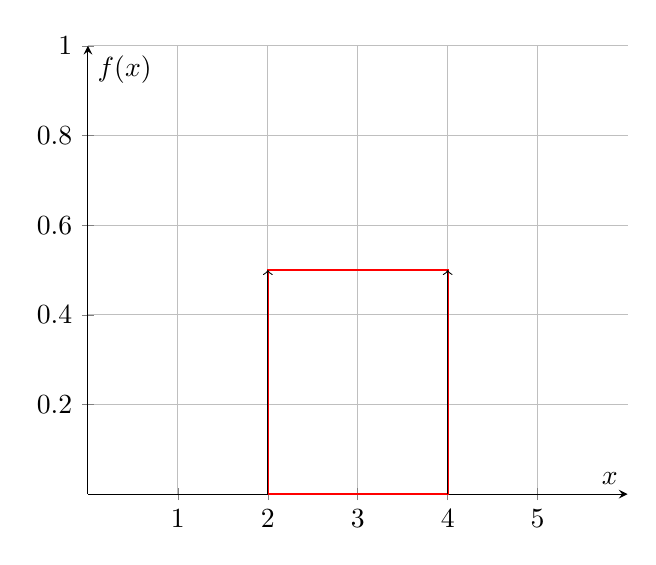
\begin{tikzpicture}
        \begin{axis}[
            axis lines = middle,
            xlabel = \( x \),
            ylabel = \( f(x) \),
            xmin = 0, xmax = 6,
            ymin = 0, ymax = 1,
            xtick={1,2,3,4,5},
            ytick={0.2,0.4,0.6,0.8,1.0},
            grid = both,
            domain=0:6,
            samples=50,
            legend pos=outer north east,
            ]
            \addplot[red, thick] coordinates {(2,0) (2,0.5) (4,0.5) (4,0) (2,0)};
            \draw[->] (2,0) -- (2,0.5);
            \draw[->] (4,0) -- (4,0.5);
            \node at (2,-0.1) {2};
            \node at (4,-0.1) {4};
        \end{axis}
    \end{tikzpicture}
    \end{center}

    The width of the rectangle (i.e., \( b - a \)) determines the range of possible values. A larger range decreases the height of the PDF, thus spreading the probability over a wider area. \\

    If \( X \) and \( Y \) are independent random variables each following a Uniform Distribution \( U(a, b) \), then the distribution of \( Z = X + Y \) can be determined. The sum of two independent Uniform random variables results in a triangular distribution over the interval \([2a, 2b]\). Specifically, the PDF of \( Z \) is piecewise linear, with its peak at \( a + b \).

\subsubsection{Exponential Distribution}

The Exponential Distribution is a continuous probability distribution that is widely used to model the time until an event occurs, such as the time until failure of a machine, the time between arrivals of customers in a queue, or the time until an earthquake. Its primary motivation lies in its memoryless property, which means that the future probability of an event occurring does not depend on how much time has already elapsed.\\

The Exponential Distribution is characterized by a single parameter, $\lambda > 0$, known as the rate parameter. 

\begin{definition}
    The PDF of the Exponential Distribution is defined as follows:
\[
f(x; \lambda) = 
\begin{cases} 
\lambda e^{-\lambda x} & \text{for } x \geq 0 \\
0 & \text{for } x < 0 
\end{cases}
\]
\end{definition}

\begin{proof}
    To derive this formula, we start from the definition of the cumulative distribution function (CDF):

\[
F(x; \lambda) = P(X \leq x) = 1 - e^{-\lambda x}, \quad x \geq 0
\]

Differentiating the CDF gives us the PDF:

\[
f(x; \lambda) = \frac{d}{dx}F(x; \lambda) = \lambda e^{-\lambda x}
\]

This derivation shows how the exponential decay characterizes the time until an event occurs.
\end{proof}

The shape of the Exponential Distribution is characterized by its PDF, which is a monotonically decreasing function. 
\begin{center}
    
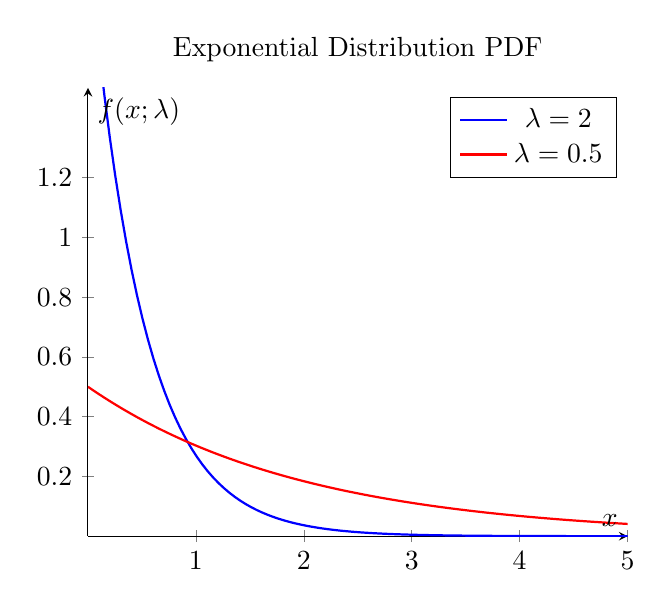
\begin{tikzpicture}
    \begin{axis}[
        axis lines=middle,
        xlabel={$x$},
        ylabel={$f(x; \lambda)$},
        title={Exponential Distribution PDF},
        ymin=0, ymax=1.5,
        xmin=0, xmax=5,
        xtick={0,1,2,3,4,5},
        ytick={0,0.2,0.4,0.6,0.8,1.0,1.2},
        domain=0:5,
        samples=100,
    ]
    \addplot[blue, thick] {2*exp(-2*x)}; % For λ = 2
    \addlegendentry{$\lambda = 2$}
    
    \addplot[red, thick] {0.5*exp(-0.5*x)}; % For λ = 0.5
    \addlegendentry{$\lambda = 0.5$}
    \end{axis}
    \end{tikzpicture}
\end{center}

The parameter $\lambda$ significantly impacts the shape of the distribution:
\begin{itemize}
    \item A larger $\lambda$ results in a steeper decline, meaning events occur more frequently (shorter waiting times).
    \item A smaller $\lambda$ leads to a slower decline, indicating longer waiting times between events.
\end{itemize}

For example, with $\lambda = 2$, the average time until the next event is $\frac{1}{2} = 0.5$ units of time, while with $\lambda = 0.5$, it is $\frac{1}{0.5} = 2$ units of time.\\

If $X$ and $Y$ are independent random variables that follow an Exponential Distribution with the same parameter $\lambda$, the distribution of the sum $Z = X + Y$ follows a Gamma Distribution with shape parameter $k = 2$ and scale parameter $\theta = \frac{1}{\lambda}$:

\[
Z \sim \text{Gamma}(k=2, \theta=\frac{1}{\lambda})
\]

The PDF of $Z$ is given by:

\[
f_Z(z; \lambda) = \frac{\lambda^2 z e^{-\lambda z}}{1!}, \quad z \geq 0
\]

We will look at the Gamma Distribution shortly. 

\begin{example}
    Consider a scenario where a factory produces light bulbs, and the average lifespan of a bulb is 1000 hours, which means $\lambda = \frac{1}{1000}$ hours$^{-1}$. \\

If we want to model the time until the next bulb fails, we use the Exponential Distribution. The probability that a bulb will last more than 1200 hours is calculated as follows:

\[
P(X > 1200) = 1 - P(X \leq 1200) = 1 - F(1200; \lambda) = e^{-\frac{1200}{1000}} \approx e^{-1.2} \approx 0.3012
\]

This means there is approximately a 30.12\% chance that the bulb will last longer than 1200 hours.

\end{example}

\subsubsection{Normal Distribution}

The Normal Distribution, also known as the Gaussian distribution, is fundamental in statistics and probability theory. It is crucial for modeling phenomena that tend to cluster around a mean. Many natural occurrences—like heights, test scores, and measurement errors—are often normally distributed. \\

The Normal Distribution is characterized by two parameters:
\begin{itemize}
    \item $\mu$: The mean, which indicates the center of the distribution.
    \item $\sigma$: The standard deviation, which measures the dispersion or spread of the distribution.
\end{itemize}
These parameters define the behavior of the distribution and its shape.

\begin{definition}
    The PDF of a Normal Distribution is given by:
\[
f(x) = \frac{1}{\sigma \sqrt{2\pi}} e^{-\frac{(x - \mu)^2}{2\sigma^2}}
\]
\end{definition}

\begin{proof}
    The PDF must satisfy two properties:
\begin{enumerate}
    \item It is non-negative: \(f(x) \geq 0\) for all \(x\).
    \item It integrates to one over the entire space:
    \[
    \int_{-\infty}^{\infty} f(x) \, dx = 1
    \]
\end{enumerate}

We want a function \(f(x)\) such that it is symmetric on both sides of its mean, allows straightforward integration, decays quickly after the mean - preferably exponentially. The function that fits these criteria is $f(x) = A e^{-B(x - \mu)^2}$. It's a bell-curve and a good choice because the shape produced by the exponential function is bell-like, which is a natural representation of many real-world phenomena that cluster around a central value. In various fields, such as physics and natural sciences, phenomena like diffusion and heat conduction can be modeled using exponential decay. This physical foundation supports the choice of the exponential function for representing distributions that describe natural processes.\\

To satisfy the normalization condition, we need:

\[
\int_{-\infty}^{\infty} A e^{-B(x - \mu)^2} \, dx = 1
\]

Changing variables to \(z = x - \mu\), we have:

\[
\int_{-\infty}^{\infty} A e^{-Bz^2} \, dz = 1
\]

This integral is known as the Gaussian integral:

\[
\int_{-\infty}^{\infty} e^{-Bz^2} \, dz = \sqrt{\frac{\pi}{B}}
\]

Thus, we have:

\[
A \sqrt{\frac{\pi}{B}} = 1 \implies A = \sqrt{\frac{B}{\pi}}
\]

Let \(B = \frac{1}{2\sigma^2}\):

\[
f(x) = \sqrt{\frac{1}{2\pi \sigma^2}} e^{-\frac{(x - \mu)^2}{2\sigma^2}}
\]

This satisfies the normalization condition. Finally, we express the PDF in its standard form:

\[
f(x) = \frac{1}{\sigma \sqrt{2\pi}} e^{-\frac{(x - \mu)^2}{2\sigma^2}}
\]
\end{proof}

\begin{definition}
    The standard normal curve is a special case of the normal distribution where the mean \(\mu\) is \(0\) and the standard deviation \(\sigma\) is \(1\). It is denoted as \(N(0, 1)\) and is symmetrical about the mean. The equation of the standard normal distribution is given by:

    \[
f(z) = \frac{1}{\sqrt{2\pi}} e^{-\frac{z^2}{2}}
\]

where \(z\) represents the z-score.
\end{definition}

\begin{definition}
    A z-score indicates how many standard deviations an element is from the mean of the distribution. It is calculated using the formula:

\[
z = \frac{(X - \mu)}{\sigma}
\]

where:
\begin{itemize}
    \item \(X\) is the value of the observation,
    \item \(\mu\) is the mean of the distribution,
    \item \(\sigma\) is the standard deviation.
\end{itemize}
\end{definition}

A positive z-score indicates that the value is above the mean, while a negative z-score indicates that it is below the mean. The z-score is crucial for standardizing values from different normal distributions to the standard normal distribution, allowing for comparison across different datasets.\\

The Normal Distribution is symmetric and bell-shaped. Its key characteristics include:
\begin{itemize}
    \item \textbf{Mean ($\mu$)}: The peak of the bell curve.
    \item \textbf{Standard Deviation ($\sigma$)}: Determines the width of the curve. A smaller $\sigma$ results in a steeper curve, while a larger $\sigma$ produces a flatter curve.
\end{itemize}

\begin{center}
    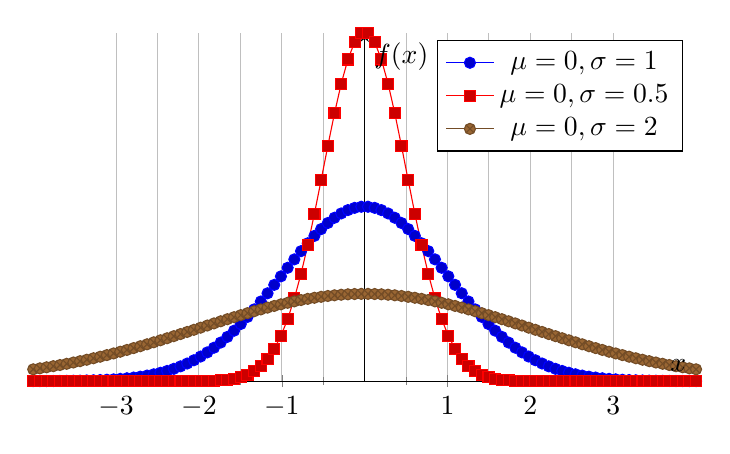
\begin{tikzpicture}
        \begin{axis}[
            axis lines = middle,
            xlabel = $x$,
            ylabel = {$f(x)$},
            xtick={-3,-2,-1,0,1,2,3},
            ytick=\empty,
            domain=-4:4,
            samples=100,
            width=10cm,
            height=6cm,
            grid=both,
            minor tick num=1,
            ]
            % Normal Distribution with mu = 0, sigma = 1
            \addplot {1/(sqrt(2*pi)*1) * exp(-((x-0)^2)/(2*1^2))};
            \addlegendentry{$\mu=0, \sigma=1$}
            
            % Normal Distribution with mu = 0, sigma = 0.5
            \addplot {1/(sqrt(2*pi)*0.5) * exp(-((x-0)^2)/(2*0.5^2))};
            \addlegendentry{$\mu=0, \sigma=0.5$}
            
            % Normal Distribution with mu = 0, sigma = 2
            \addplot {1/(sqrt(2*pi)*2) * exp(-((x-0)^2)/(2*2^2))};
            \addlegendentry{$\mu=0, \sigma=2$}
            
        \end{axis}
    \end{tikzpicture}
    \end{center}

The graph illustrates the effect of varying standard deviations on the distribution's shape. For example:
\begin{itemize}
    \item When $\sigma = 0.5$, the distribution is narrow and peaked.
    \item When $\sigma = 2$, the distribution is wider and flatter.
\end{itemize} 

If \(X\) and \(Y\) are independent random variables, both following a Normal Distribution:
\[
X \sim N(\mu_X, \sigma_X^2), \quad Y \sim N(\mu_Y, \sigma_Y^2)
\]
Then, the sum \(Z = X + Y\) is also normally distributed:
\[
Z \sim N(\mu_X + \mu_Y, \sigma_X^2 + \sigma_Y^2)
\]

\begin{example}
    Suppose the heights of adult men in a certain city are normally distributed with a mean of \(\mu = 175\) cm and a standard deviation of \(\sigma = 10\) cm. \\

Calculate the following:
\begin{enumerate}
    \item The z-score for a man who is 190 cm tall.
    \item The probability that a randomly selected man from this city is taller than 190 cm.
\end{enumerate}

The z-score is calculated using the formula:

\[
z = \frac{(X - \mu)}{\sigma}
\]

where:
\begin{itemize}
    \item \(X\) is the value for which we want to find the z-score,
    \item \(\mu\) is the mean,
    \item \(\sigma\) is the standard deviation.
\end{itemize}

For a man who is \(X = 190\) cm tall:

\[
z = \frac{(190 - 175)}{10} = \frac{15}{10} = 1.5
\]

To find the probability that a randomly selected man is taller than 190 cm, we look up the z-score in the standard normal distribution table or use a cumulative distribution function (CDF) calculator. \\

The CDF gives the probability that a random variable is less than a certain value. Thus, we need to find:

\[
P(X > 190) = 1 - P(X \leq 190) = 1 - P(Z \leq 1.5)
\]

From standard normal distribution tables, we find:

\[
P(Z \leq 1.5) \approx 0.9332
\]

Therefore, the probability is:

\[
P(X > 190) = 1 - 0.9332 = 0.0668
\]

The z-score for a man who is 190 cm tall is \(1.5\), and the probability that a randomly selected man from this city is taller than 190 cm is approximately \(0.0668\), or \(6.68\%\).

\end{example}

\subsubsection{Log-Normal Distribution}

The Log-Normal distribution is a continuous probability distribution of a random variable whose logarithm is normally distributed. It is commonly used to model variables that are multiplicative in nature, such as stock prices, income distributions, and the sizes of living organisms. \\

The primary parameters involved in modeling a Log-Normal distribution are:
\begin{itemize}
    \item $\mu$: the mean of the underlying normal distribution (i.e., the logarithm of the variable).
    \item $\sigma$: the standard deviation of the underlying normal distribution.
\end{itemize}

\begin{definition}
    The PDF of the Log-Normal distribution is defined as follows:
\[
f(x; \mu, \sigma) = \frac{1}{x \sigma \sqrt{2\pi}} e^{-\frac{(\ln x - \mu)^2}{2\sigma^2}}, \quad x > 0
\]
\end{definition}

\begin{proof}
    We start from the fact that if \( Y \) is normally distributed, i.e., \( Y \sim N(\mu, \sigma^2) \), then the random variable \( X = e^Y \) follows a Log-Normal distribution. The transformation of variables provides us with the PDF. Start with the PDF of normal distribution:

    \[
f_Y(y) = \frac{1}{\sigma \sqrt{2\pi}} e^{-\frac{(y - \mu)^2}{2\sigma^2}}
\]

Apply the transformation \( x = e^y \), which implies \( y = \ln x \) and \( dy = \frac{1}{x} dx \).\\

The PDF of \( X \) is then obtained using the change of variable:
\[
f_X(x) = f_Y(\ln x) \cdot \left| \frac{dy}{dx} \right| = f_Y(\ln x) \cdot \frac{1}{x}
\]

Substituting \( f_Y(\ln x) \) yields the PDF of the Log-Normal distribution as stated above.
\end{proof}

The shape of the Log-Normal distribution is positively skewed, meaning it has a long tail on the right side. The parameters $\mu$ and $\sigma$ significantly impact its shape:

\begin{itemize}
    \item As $\mu$ increases, the peak of the distribution shifts to the right, indicating a higher central tendency.
    \item An increase in $\sigma$ increases the spread of the distribution, resulting in a wider and flatter shape. Conversely, a smaller $\sigma$ leads to a steeper peak.
\end{itemize}

\begin{center}
    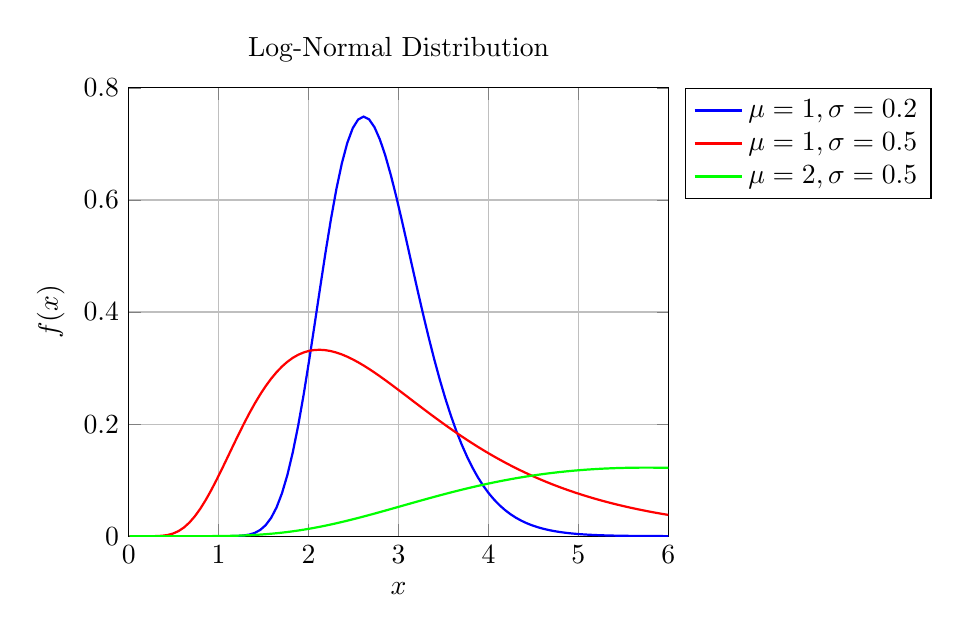
\begin{tikzpicture}
        \begin{axis}[
            title={Log-Normal Distribution},
            xlabel={$x$},
            ylabel={$f(x)$},
            xmin=0, xmax=6,
            ymin=0, ymax=0.8,
            legend pos=outer north east,
            grid=major,
            domain=0.01:6,
            samples=100
        ]
        \addplot[blue, thick] {1/(x*0.2*sqrt(2*pi))*exp(-((ln(x)-1)^2)/(2*0.2^2))}; 
        \addlegendentry{$\mu=1, \sigma=0.2$}
    
        \addplot[red, thick] {1/(x*0.5*sqrt(2*pi))*exp(-((ln(x)-1)^2)/(2*0.5^2))}; 
        \addlegendentry{$\mu=1, \sigma=0.5$}
    
        \addplot[green, thick] {1/(x*0.5*sqrt(2*pi))*exp(-((ln(x)-2)^2)/(2*0.5^2))}; 
        \addlegendentry{$\mu=2, \sigma=0.5$}
        \end{axis}
    \end{tikzpicture}
    \end{center}

    For example, with $\mu = 1$ and $\sigma = 0.2$, the distribution is relatively concentrated around the mean, while with $\sigma = 0.5$, it spreads out more, showing the impact of increasing variance.\\

    If \( X \) and \( Y \) are independent random variables that follow a Log-Normal distribution, specifically \( X \sim \text{Log-Normal}(\mu_X, \sigma_X^2) \) and \( Y \sim \text{Log-Normal}(\mu_Y, \sigma_Y^2) \), the distribution of the sum \( Z = X + Y \) does not follow a Log-Normal distribution. \\

However, there are approximations to understand the distribution of \( Z \). In some cases, the sum of two Log-Normal random variables can be approximated using a Normal distribution or simulated using numerical methods, depending on the parameters.

\begin{example}
    Consider the modeling of the future price of a stock that currently has a price of $P_0 = 100$. Assuming that the logarithm of the price follows a Normal distribution with parameters \( \mu = 0.05 \) and \( \sigma = 0.1 \):\\

1. We simulate the future price of the stock after 1 year:
\[
P = P_0 \cdot e^{Y}
\]
where \( Y \sim N(0.05, 0.1^2) \).\\

2. If we calculate the expected price and the variance, we can understand the distribution of future prices.\\

This modeling helps investors understand the risks and potential returns associated with stock investments, providing a probabilistic framework for decision-making.
\end{example}

\subsubsection{Weibull Distribution}

The Weibull distribution is a continuous probability distribution that is widely used in reliability analysis and failure time analysis. It is particularly useful in modeling life data, where it can describe the time until an event occurs, such as failure of a mechanical component or time to death in survival studies.\\

\begin{definition}
    The PDF of the Weibull distribution is given by:

\[
f(x; k, \lambda) = 
\begin{cases} 
\frac{k}{\lambda} \left( \frac{x}{\lambda} \right)^{k-1} e^{-(x/\lambda)^{k}} & \text{for } x \geq 0 \\
0 & \text{for } x < 0 
\end{cases}
\]
\end{definition}

\begin{proof}
    To derive this PDF, we start with the cumulative distribution function (CDF), defined as:

\[
F(x; k, \lambda) = 1 - e^{-(x/\lambda)^{k}} \quad \text{for } x \geq 0
\]

Taking the derivative of the CDF with respect to $x$ yields the PDF:

\[
f(x; k, \lambda) = \frac{d}{dx} F(x; k, \lambda) = \frac{d}{dx} \left( 1 - e^{-(x/\lambda)^{k}} \right) = \frac{k}{\lambda} \left( \frac{x}{\lambda} \right)^{k-1} e^{-(x/\lambda)^{k}}
\]
\end{proof}

The shape of the Weibull distribution is heavily influenced by the shape parameter $k$:

\begin{itemize}
    \item If $k < 1$: The distribution is decreasing; it indicates that the failure rate decreases over time (e.g., "infant mortality").
    \item If $k = 1$: The distribution is exponential, implying a constant failure rate.
    \item If $k > 1$: The distribution is increasing; it indicates that the failure rate increases over time (e.g., "wear-out failures").
\end{itemize}

The scale parameter $\lambda$ stretches or compresses the distribution along the x-axis. A larger $\lambda$ results in a distribution that spreads out more, while a smaller $\lambda$ makes it steeper.

\begin{center}
    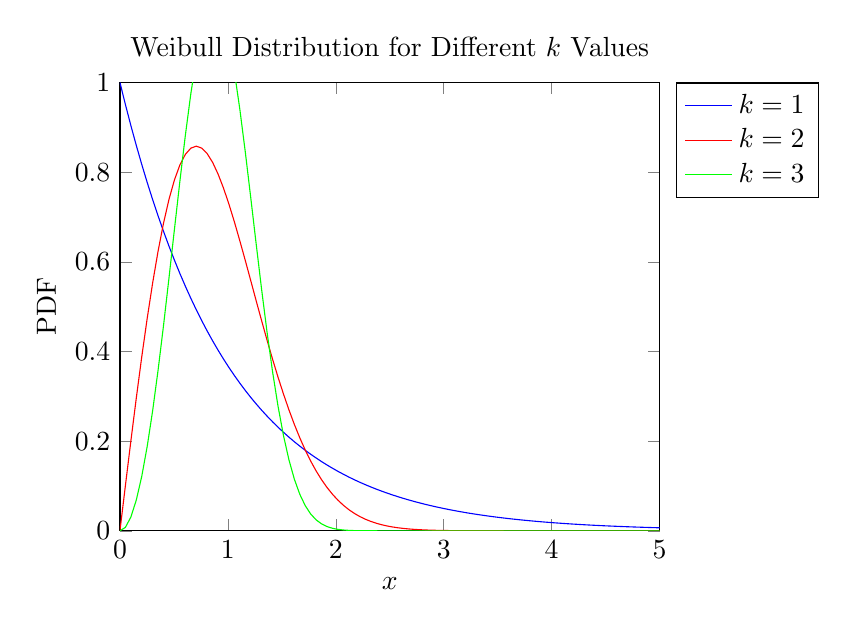
\begin{tikzpicture}
        \begin{axis}[
            xlabel={$x$},
            ylabel={PDF},
            xmin=0, xmax=5,
            ymin=0, ymax=1,
            title={Weibull Distribution for Different $k$ Values},
            legend pos=outer north east,
            samples=100
        ]
        \addplot[domain=0:5, color=blue]{(1/1) * (x/1)^(1-1) * exp(-(x/1)^1)};
        \addlegendentry{$k=1$}
        
        \addplot[domain=0:5, color=red]{(2/1) * (x/1)^(2-1) * exp(-(x/1)^2)};
        \addlegendentry{$k=2$}
        
        \addplot[domain=0:5, color=green]{(3/1) * (x/1)^(3-1) * exp(-(x/1)^3)};
        \addlegendentry{$k=3$}
        \end{axis}
    \end{tikzpicture}
    \end{center}

    In this graph, we see the differences in the shapes for $k=1$, $k=2$, and $k=3$.\\

    If $X$ and $Y$ are independent random variables following the Weibull distribution with the same scale parameter $\lambda$ and shape parameter $k$, the distribution of $X + Y$ is not generally a Weibull distribution. However, if both are identically distributed, we can use techniques such as convolution to find the PDF of $Z = X + Y$. The resulting distribution would require numerical methods for specific parameters and is generally not expressible in a closed form.

    \begin{example}
        Suppose the shape parameter is found to be $k=1.5$ and the scale parameter is $\lambda=1000$ hours. This indicates that the bulbs experience increasing failure rates as time progresses. The company can use this model to predict the reliability of their bulbs, estimating that approximately 63\% of the bulbs will have failed by 1000 hours.
    \end{example}

\subsubsection{Gamma Distribution}

The Gamma distribution is a continuous probability distribution that is widely used to model various processes, particularly those that involve waiting times or the time until an event occurs. Its flexibility makes it suitable for a variety of applications, including queuing models, reliability analysis, and Bayesian statistics.\\

The Gamma distribution is characterized by two parameters: 
\begin{itemize}
    \item \(\alpha\) (shape parameter): This parameter dictates the shape of the distribution. It is a positive real number that influences the skewness and the peak of the distribution.
    \item \(\beta\) (rate parameter): This parameter is also a positive real number, and it controls the scale of the distribution. It is often expressed as the reciprocal of the scale parameter \(\theta\) (where \(\theta = \frac{1}{\beta}\)).
\end{itemize}

Before diving into the Gamma distribution, it is essential to understand the Gamma function, which is defined as:
\[
\Gamma(n) = \int_0^\infty t^{n-1} e^{-t} \, dt
\]
for \( n > 0 \). The Gamma function generalizes the factorial function to real and complex numbers, with the relationship:
\[
\Gamma(n) = (n-1)!
\]
for natural numbers \( n \). The derivation of the Gamma function arises from the need to extend the concept of factorial to non-integer values, facilitating calculations in various mathematical fields, particularly in calculus and complex analysis.

\begin{definition}
    The PDF of the Gamma distribution is given by:
\[
f(x; \alpha, \beta) = \frac{\beta^\alpha}{\Gamma(\alpha)} x^{\alpha-1} e^{-\beta x}, \quad x > 0
\]
where \(\Gamma(\alpha)\) is the Gamma function.
\end{definition}

Before we dive into the proof of this PDF, we will need some results. 

\begin{theorem}
    The PDF of the sum of two independent random variables is the convolution of their PDFs. 
\end{theorem}

\begin{proof}
    Let \(Z = X + Y\). We want to find the PDF \(f_Z(z)\) of the random variable \(Z\).\\

    To derive \(f_Z(z)\), we can first find the cumulative distribution function (CDF) \(F_Z(z)\):
\[
F_Z(z) = P(Z \leq z) = P(X + Y \leq z).
\]

Given the independence of \(X\) and \(Y\), we can express the probability \(P(X + Y \leq z)\) as:
\[
F_Z(z) = \int_{-\infty}^{\infty} P(X \leq z - y) f_Y(y) \, dy.
\]

Here, \(P(X \leq z - y)\) is the CDF of \(X\), denoted by \(F_X(z - y)\):
\[
F_Z(z) = \int_{-\infty}^{\infty} F_X(z - y) f_Y(y) \, dy.
\]

To find the PDF \(f_Z(z)\), we differentiate \(F_Z(z)\) with respect to \(z\):
\[
f_Z(z) = \frac{d}{dz} F_Z(z) = \frac{d}{dz} \int_{-\infty}^{\infty} F_X(z - y) f_Y(y) \, dy.
\]

Using the Leibniz rule for differentiating under the integral sign, we have:
\[
f_Z(z) = \int_{-\infty}^{\infty} \frac{\partial}{\partial z} F_X(z - y) f_Y(y) \, dy.
\]

Since \(F_X(z - y)\) is the CDF of \(X\), its derivative is the PDF \(f_X(z - y)\):
\[
\frac{\partial}{\partial z} F_X(z - y) = f_X(z - y).
\]

Thus,
\[
f_Z(z) = \int_{-\infty}^{\infty} f_X(z - y) f_Y(y) \, dy.
\]

The expression we derived for \(f_Z(z)\) is the convolution of the PDFs \(f_X\) and \(f_Y\):
\[
f_Z(z) = (f_X * f_Y)(z) = \int_{-\infty}^{\infty} f_X(z - y) f_Y(y) \, dy.
\]

Therefore, we have shown that the PDF of the sum of two independent random variables \(Z = X + Y\) can be found using the convolution of their PDFs:
\[
f_Z(z) = f_X(z) * f_Y(z).
\]
\end{proof}

Now we can prove the PDF of the Gamma Distribution. The Gamma Distribution should be viewed as the Sum of Independent Exponential Random Variables. Let's prove this. 

\begin{proof}
    Let \(X_1, X_2, \ldots, X_k\) be \(k\) independent random variables, each following an exponential distribution with rate \(\beta\). The PDF of each \(X_i\) is given by:
\[
f_{X_i}(x) = \beta e^{-\beta x}, \quad x \geq 0.
\]

Define \(Y = X_1 + X_2 + \ldots + X_k\). We want to find the PDF of \(Y\).\\

The PDF of the sum of two independent random variables can be found using the convolution of their PDFs. The convolution of two PDFs \(f_X(x)\) and \(f_Y(y)\) is defined as:
\[
(f_X * f_Y)(z) = \int_0^z f_X(x) f_Y(z - x) \, dx.
\]

First, we find the PDF of \(Z = X_1 + X_2\):
\[
f_Z(z) = \int_0^z f_{X_1}(x) f_{X_2}(z - x) \, dx.
\]
Substituting the PDFs of the exponential distributions:
\[
f_Z(z) = \int_0^z \beta e^{-\beta x} \cdot \beta e^{-\beta (z - x)} \, dx.
\]
This simplifies to:
\[
f_Z(z) = \beta^2 e^{-\beta z} \int_0^z dx = \beta^2 e^{-\beta z} \cdot z.
\]
Thus,
\[
f_Z(z) = \beta^2 z e^{-\beta z}, \quad z \geq 0.
\]

Now, let's generalize this for \(k\) independent exponential random variables. We can derive it step by step:
1. Assume \(Y_k = X_1 + X_2 + \ldots + X_k\).
2. We already have the result for \(k=2\):
   \[
   f_{Y_2}(y) = \beta^2 y e^{-\beta y}.
   \]

Now, using the result for \(k=2\), we find the PDF of \(Y_k\) as follows:
\[
f_{Y_k}(y) = \int_0^y f_{Y_{k-1}}(x) f_{X_k}(y - x) \, dx.
\]
Substituting \(f_{Y_{k-1}}(x)\) and \(f_{X_k}(y - x)\):
\[
f_{Y_k}(y) = \int_0^y \left( \frac{\beta^{k-1}}{\Gamma(k-1)} x^{k-2} e^{-\beta x} \right) \left( \beta e^{-\beta (y - x)} \right) \, dx.
\]
This simplifies to:
\[
f_{Y_k}(y) = \beta^k e^{-\beta y} \int_0^y \frac{x^{k-2}}{\Gamma(k-1)} \, dx.
\]
The integral evaluates to:
\[
\int_0^y x^{k-2} \, dx = \frac{y^{k-1}}{k-1}.
\]
Thus, we have:
\[
f_{Y_k}(y) = \beta^k e^{-\beta y} \cdot \frac{y^{k-1}}{\Gamma(k)}.
\]
Thus, the PDF of \(Y = X_1 + X_2 + \ldots + X_k\) is given by:
\[
f_Y(y) = \frac{\beta^k}{\Gamma(k)} y^{k-1} e^{-\beta y}, \quad y \geq 0.
\]

This is the PDF of the Gamma distribution with shape parameter \(k\) and rate parameter \(\beta\). Therefore, we have proven that the Gamma distribution can be viewed as the sum of \(k\) independent exponentially distributed random variables.
\end{proof}

The shape of the Gamma distribution is highly influenced by its parameters \(\alpha\) and \(\beta\). 

\begin{itemize}
    \item For \(\alpha = 1\): The Gamma distribution simplifies to an exponential distribution, characterized by a single peak.
    \item For \(\alpha > 1\): The distribution becomes increasingly bell-shaped, with the peak shifting to the right as \(\alpha\) increases.
    \item For \(\alpha < 1\): The distribution is skewed to the right, approaching zero as \(x\) increases.
\end{itemize}

\begin{center}
    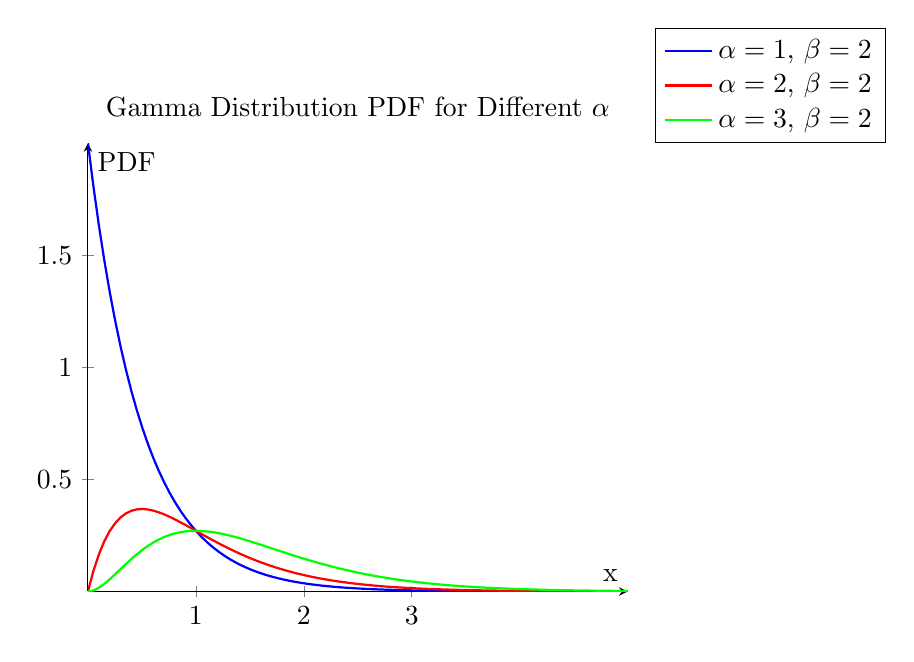
\begin{tikzpicture}
        \begin{axis}[
            axis lines = middle,
            xlabel = {x},
            ylabel = {PDF},
            xtick={0,1,2,3},
            ytick={0,0.5,1,1.5},
            domain=0:5,
            samples=100,
            legend style={at={(1.05,1)},anchor=south west},
            title={Gamma Distribution PDF for Different $\alpha$}
        ]
        \addplot[blue, thick] {2*exp(-2*x)}; % alpha = 1
        \addlegendentry{$\alpha = 1$, $\beta = 2$}
        
        \addplot[red, thick] {0.5*2^2*x*exp(-2*x)}; % alpha = 2
        \addlegendentry{$\alpha = 2$, $\beta = 2$}
        
        \addplot[green, thick] {0.5*2^3*x^2*exp(-2*x)/2}; % alpha = 3
        \addlegendentry{$\alpha = 3$, $\beta = 2$}
        \end{axis}
    \end{tikzpicture}
    \end{center}

    If \(X\) and \(Y\) are independent random variables each following a Gamma distribution with parameters \((\alpha_1, \beta)\) and \((\alpha_2, \beta)\) respectively, then the distribution of \(X + Y\) is given by:
    \[
    X + Y \sim \Gamma(\alpha_1 + \alpha_2, \beta)
    \]
    This property is significant in various applications, such as queuing theory, where the total waiting time can be modeled using the sum of Gamma-distributed random variables.

    \begin{example}
        Suppose a call center receives calls according to a Poisson process with an average rate of \(\lambda = 5\) calls per hour. The waiting time until the \(k\)-th call can be modeled using a Gamma distribution. \\

If we want to find the distribution of the waiting time for the 3rd call (\(X \sim \Gamma(3, \lambda)\)), we can determine the expected waiting time as:
\[
E[X] = \frac{\alpha}{\beta} = \frac{3}{5} = 0.6 \text{ hours} \quad (\text{or } 36 \text{ minutes})
\]
In this scenario, the Gamma distribution helps assess service times and manage resource allocation effectively.
    \end{example}

\subsubsection{Beta Distribution}

The Beta distribution is a continuous probability distribution defined on the interval \([0, 1]\). It is particularly useful in modeling random variables that represent proportions or probabilities. The motivation behind the Beta distribution arises from the need to model outcomes that are constrained within a finite range. The Beta distribution has widespread applications, particularly in Bayesian statistics, project management (e.g., PERT charts), and quality control. For instance, in project management, the Beta distribution can model the completion time of a project where the completion time is uncertain. \\

The Beta distribution is characterized by two shape parameters, \(\alpha\) and \(\beta\), which control the distribution's shape. The parameters represent the number of successes and failures, respectively, in a binomial distribution. Before delving into the Beta distribution, it's essential to understand the Beta function, which serves as the normalization constant for the Beta distribution. \\

The Beta function, denoted as \(B(x, y)\), is defined as:

\[
B(x, y) = \int_0^1 t^{x-1} (1 - t)^{y-1} dt
\]

This integral arises in various areas of mathematics, particularly in calculus and combinatorial analysis. The Beta function can be related to the Gamma function via the identity:

\[
B(x, y) = \frac{\Gamma(x) \Gamma(y)}{\Gamma(x + y)}
\]

The Beta function is used to normalize the Beta distribution, ensuring that the total area under the probability density function (PDF) equals 1.

\begin{definition}
    The PDF of the Beta distribution is given by:

\[
f(x; \alpha, \beta) = \frac{x^{\alpha - 1} (1 - x)^{\beta - 1}}{B(\alpha, \beta)} \quad \text{for } 0 < x < 1
\]

where \(\alpha > 0\) and \(\beta > 0\).
\end{definition}

\begin{proof}
    The PDF of the Beta distribution, denoted as \(f(x; \alpha, \beta)\), can be expressed as a function that needs to be normalized. We propose a form:

\[
f(x; \alpha, \beta) = C \cdot x^{\alpha - 1} (1 - x)^{\beta - 1}
\]

where \(C\) is a normalization constant.\\

To ensure that the PDF integrates to 1 over the interval \([0, 1]\), we must have:

\[
\int_0^1 f(x; \alpha, \beta) \, dx = 1
\]

Substituting our proposed form into this equation gives:

\[
\int_0^1 C \cdot x^{\alpha - 1} (1 - x)^{\beta - 1} \, dx = 1
\]

We recognize the left-hand side as the definition of the Beta function:

\[
C \cdot B(\alpha, \beta) = 1
\]

Thus, we find the normalization constant \(C\):

\[
C = \frac{1}{B(\alpha, \beta)}
\]

Substituting \(C\) back into our proposed PDF gives:

\[
f(x; \alpha, \beta) = \frac{1}{B(\alpha, \beta)} \cdot x^{\alpha - 1} (1 - x)^{\beta - 1}
\]
\end{proof}

The shape of the Beta distribution can vary significantly depending on the parameters \(\alpha\) and \(\beta\):

\begin{itemize}
    \item If \(\alpha = 1\) and \(\beta = 1\), the distribution is uniform on \([0, 1]\).
    \item If \(\alpha > 1\) and \(\beta = 1\), the distribution is increasing.
    \item If \(\alpha = 1\) and \(\beta > 1\), the distribution is decreasing.
    \item If \(\alpha > 1\) and \(\beta > 1\), the distribution is bell-shaped, peaking around \(\frac{\alpha - 1}{\alpha + \beta - 2}\).
    \item If \(\alpha < 1\) and \(\beta < 1\), the distribution has U-shape.
\end{itemize}

\begin{center}
    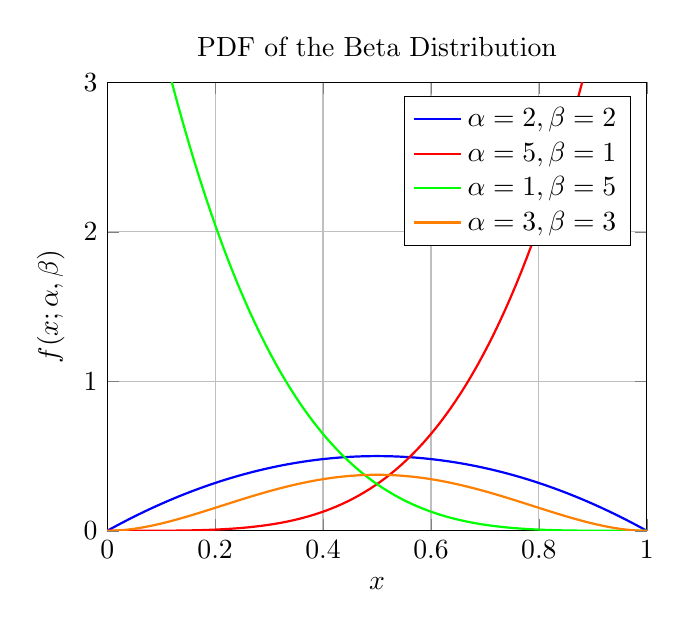
\begin{tikzpicture}
        \begin{axis}[
            xlabel={$x$},
            ylabel={$f(x; \alpha, \beta)$},
            xmin=0, xmax=1,
            ymin=0, ymax=3,
            domain=0:1,
            samples=100,
            legend pos=north east,
            grid=major,
            title={PDF of the Beta Distribution}
        ]
            % Plot for alpha = 2, beta = 2
            \addplot[blue, thick] {2 * x * (1 - x)};
            \addlegendentry{$\alpha = 2, \beta = 2$}
            
            % Plot for alpha = 5, beta = 1
            \addplot[red, thick] {5 * x^4};
            \addlegendentry{$\alpha = 5, \beta = 1$}
            
            % Plot for alpha = 1, beta = 5
            \addplot[green, thick] {5 * (1 - x)^4};
            \addlegendentry{$\alpha = 1, \beta = 5$}
            
            % Plot for alpha = 3, beta = 3
            \addplot[orange, thick] {6 * x^2 * (1 - x)^2};
            \addlegendentry{$\alpha = 3, \beta = 3$}
        \end{axis}
    \end{tikzpicture}
\end{center}

For example, when \(\alpha = 2\) and \(\beta = 2\), the distribution is symmetric around \(0.5\), while \(\alpha = 0.5\) and \(\beta = 0.5\) create a U-shaped distribution.\\

If \(X\) and \(Y\) are independent random variables that follow a Beta distribution, specifically \(X \sim \text{Beta}(\alpha_1, \beta_1)\) and \(Y \sim \text{Beta}(\alpha_2, \beta_2)\), the distribution of \(X + Y\) does not follow a standard distribution. However, under specific conditions (e.g., when both variables are scaled), the result can be approximated or analyzed using convolution techniques.\\

In general, the sum of two Beta variables requires numerical methods or simulations for precise analysis.

\begin{example}
    Suppose we have a project that requires three estimates: optimistic time (5 days), pessimistic time (15 days), and most likely time (10 days). We can use the Beta distribution to model the likelihood of completing the project within a certain timeframe. \\

    Let \(\alpha\) and \(\beta\) be determined based on these estimates using the formula:

\[
\alpha = \frac{(m - a)(b - m)}{(b - a)^2}, \quad \beta = \frac{(b - m)(m - a)}{(b - a)^2}
\]

where \(m\) is the most likely time, \(a\) is the optimistic time, and \(b\) is the pessimistic time.\\

In this case, the application of the Beta distribution helps project managers evaluate risk and optimize project timelines based on uncertainty.
\end{example}

\subsubsection{Chi-squared Distribution}
The Chi-squared distribution is a continuous probability distribution that arises in statistical inference, particularly in hypothesis testing and confidence interval estimation for population variance. It is commonly used to model the distribution of the sum of the squares of $k$ independent standard normal random variables. \\

To understand the motivation behind the Chi-squared distribution, consider that many statistical tests rely on estimating variances from sample data. When you collect data and calculate how far each data point is from the mean, you are effectively measuring variability. The Chi-squared distribution helps us determine whether the observed variability in our sample data is consistent with a certain population variance or if it indicates something unusual.\\

The parameters involved in this modeling include:
\begin{itemize}
    \item The number of degrees of freedom ($k$), which corresponds to the number of independent standard normal variables being squared and summed.
\end{itemize}

\begin{definition}
    The PDF of the Chi-squared distribution with $k$ degrees of freedom is given by:
\[
f(x; k) = \frac{1}{2^{k/2} \Gamma(k/2)} x^{(k/2)-1} e^{-x/2}, \quad \text{for } x > 0
\]
where $\Gamma$ is the Gamma function.
\end{definition}

\begin{proof}
    The Chi-squared distribution is defined as the distribution of the sum of the squares of $k$ independent standard normal random variables. This derivation will illustrate how we arrive at the probability density function (PDF) of the Chi-squared distribution.\\

    Let $Z \sim N(0, 1)$ be a standard normal random variable, which has the following PDF:
\[
f_Z(z) = \frac{1}{\sqrt{2\pi}} e^{-\frac{z^2}{2}}, \quad \text{for } -\infty < z < \infty.
\]

Consider $k$ independent standard normal random variables:
\[
Z_1, Z_2, \ldots, Z_k \sim N(0, 1.
\]
The Chi-squared variable is defined as:
\[
Y = Z_1^2 + Z_2^2 + \ldots + Z_k^2.
\]

To find the PDF of $Y$, we start with the joint distribution of the $Z_i$. The joint PDF of $Z_1, Z_2, \ldots, Z_k$ is given by:
\[
f_{Z_1, Z_2, \ldots, Z_k}(z_1, z_2, \ldots, z_k) = \prod_{i=1}^{k} f_Z(z_i) = \left(\frac{1}{\sqrt{2\pi}}\right)^k e^{-\frac{1}{2} \sum_{i=1}^{k} z_i^2}.
\]

Next, we make a change of variables from $Z_1, Z_2, \ldots, Z_k$ to $Y$ and the angles in polar coordinates, where:
\[
Y = Z_1^2 + Z_2^2 + \ldots + Z_k^2
\]
and the Jacobian determinant of the transformation will involve the angles.

The relationship in polar coordinates leads to:
\[
z_1^2 + z_2^2 + \ldots + z_k^2 = r^2
\]
where $r^2 = Y$. The angle terms introduce a factor of $\frac{(2\pi)^{k/2}}{(r^{k-1})}$ due to the transformation to polar coordinates.
We can then express the PDF of $Y$ as follows:
\[
f_Y(y) = \int_{\mathbb{R}^{k-1}} f_{Z_1, Z_2, \ldots, Z_k}(z_1, z_2, \ldots, z_k) \, dz_1 dz_2 \ldots dz_{k-1}.
\]
Substituting the expression for $f_{Z_1, Z_2, \ldots, Z_k}$ and integrating out the angular parts gives:
\[
f_Y(y) = \frac{1}{(2\pi)^{k/2}} \int_{0}^{2\pi} e^{-\frac{y}{2}} y^{(k/2)-1} \frac{(2\pi)^{k/2}}{(r^{k-1})} dr.
\]

After performing the integration, we arrive at:
\[
f_Y(y) = \frac{1}{2^{k/2} \Gamma(k/2)} y^{(k/2)-1} e^{-y/2}, \quad y > 0.
\]We can then express the PDF of $Y$ as follows:
\[
f_Y(y) = \int_{\mathbb{R}^{k-1}} f_{Z_1, Z_2, \ldots, Z_k}(z_1, z_2, \ldots, z_k) \, dz_1 dz_2 \ldots dz_{k-1}.
\]
Substituting the expression for $f_{Z_1, Z_2, \ldots, Z_k}$ and integrating out the angular parts gives:
\[
f_Y(y) = \frac{1}{(2\pi)^{k/2}} \int_{0}^{2\pi} e^{-\frac{y}{2}} y^{(k/2)-1} \frac{(2\pi)^{k/2}}{(r^{k-1})} dr.
\]

After performing the integration, we arrive at:
\[
f_Y(y) = \frac{1}{2^{k/2} \Gamma(k/2)} y^{(k/2)-1} e^{-y/2}, \quad y > 0.
\]Thus, we have derived the PDF of the Chi-squared distribution with $k$ degrees of freedom:
\[
f_Y(y) = \frac{1}{2^{k/2} \Gamma(k/2)} y^{(k/2)-1} e^{-y/2}, \quad y > 0.
\]
\end{proof}

The shape of the Chi-squared distribution depends significantly on the degrees of freedom ($k$):
\begin{itemize}
    \item For $k = 1$: The distribution is highly skewed to the right.
    \item For $k = 2$: The distribution starts to take on a more pronounced bell shape.
    \item As $k$ increases, the distribution becomes more symmetric and approaches a normal distribution \textit{(due to central limit theorem - will be studied later)}.
\end{itemize}

\begin{center}
    \begin{tikzpicture}
        \begin{axis}[
            title={Chi-squared Distribution},
            xlabel={$y$},
            ylabel={PDF},
            legend pos=outer north east,
            grid=major,
            domain=0:15,
            samples=100,
            ymin=0, ymax=0.4,
            unbounded coords=jump
        ]
        \addplot[blue, thick] {1/(2^(1/2)*tgamma(1/2))*x^(1/2-1)*exp(-x/2)};
        \addplot[red, thick] {1/(2^(2/2)*tgamma(2/2))*x^(2/2-1)*exp(-x/2)};
        \addplot[green, thick] {1/(2^(5/2)*tgamma(5/2))*x^(5/2-1)*exp(-x/2)};
        \legend{$k=1$, $k=2$, $k=5$}
        \end{axis}
    \end{tikzpicture}
    \end{center}

    
    For example:
    \begin{itemize}
        \item For $k = 1$, the peak is at $x = 0$, and it falls off steeply.
        \item For $k = 5$, the distribution is more spread out and has a more pronounced peak, making it resemble a normal distribution.
    \end{itemize}

    If $X \sim \chi^2(k_1)$ and $Y \sim \chi^2(k_2)$ are independent Chi-squared random variables, then the sum $Z = X + Y$ follows a Chi-squared distribution with $k_1 + k_2$ degrees of freedom:
\[
Z \sim \chi^2(k_1 + k_2)
\]

\begin{example}
    Consider a researcher testing whether a six-sided die is fair. They roll the die 60 times and record the frequency of each outcome. If the observed frequencies are significantly different from the expected frequencies (10 for each side), the researcher can use the Chi-squared test to determine whether the die is biased. The test statistic is calculated as:
\[
\chi^2 = \sum \frac{(O_i - E_i)^2}{E_i}
\]
where \(O_i\) is the observed frequency and \(E_i\) is the expected frequency. By comparing this statistic to the Chi-squared distribution with appropriate degrees of freedom, the researcher can draw conclusions about the fairness of the die.
\end{example}

\subsubsection{Student's t-Distribution}

When we collect data from a population, we often want to estimate the mean and understand the variability of that mean. However, if our sample size is small (typically less than 30), the sampling distribution of the sample mean follows a t-distribution rather than a normal distribution. \\

The parameters involved in this modeling include:
\begin{itemize}
    \item The sample size \( n \)
    \item The sample mean \( \bar{x} \)
    \item The sample standard deviation \( s \)
\end{itemize}

\begin{definition}
    The PDF of the Student's t-distribution is defined as:

\[
f(t) = \frac{\Gamma\left(\frac{v+1}{2}\right)}{\sqrt{v \pi} \, \Gamma\left(\frac{v}{2}\right)} \left(1 + \frac{t^2}{v}\right)^{-\frac{v+1}{2}}
\]

where \( v \) is the degrees of freedom and \( \Gamma \) is the gamma function.
\end{definition}

\begin{proof}
    The Student's t-distribution arises when we estimate the mean of a normally distributed population with an unknown standard deviation. To derive its probability density function (PDF), we start with the following components.\\

    Given a sample of \( n \) observations \( X_1, X_2, \ldots, X_n \), the sample mean \( \bar{X} \) and sample standard deviation \( S \) are defined as:

   \[
   \bar{X} = \frac{1}{n} \sum_{i=1}^{n} X_i,
   \]
   \[
   S = \sqrt{\frac{1}{n-1} \sum_{i=1}^{n} (X_i - \bar{X})^2}.
   \]

   The t-statistic is defined as:

   \[
   t = \frac{\bar{X} - \mu}{S / \sqrt{n}},
   \]

   where \( \mu \) is the true population mean. \\

   If the underlying population is normally distributed, the numerator \( \bar{X} - \mu \) follows a normal distribution with mean \( 0 \) and variance \( \frac{\sigma^2}{n} \), where \( \sigma^2 \) is the population variance. The denominator \( S \) is independent of \( \bar{X} \) and follows a scaled chi-squared distribution. \\

   Assuming \( X_i \) follows a normal distribution \( \mathcal{N}(\mu, \sigma^2) \):

\[
\bar{X} \sim \mathcal{N}\left(\mu, \frac{\sigma^2}{n}\right).
\]

The sample variance \( S^2 \) follows a chi-squared distribution:

\[
\frac{(n-1)S^2}{\sigma^2} \sim \chi^2_{n-1}.
\]

The joint distribution of \( \bar{X} \) and \( S^2 \) can be expressed using their independence:

\[
f_{\bar{X}, S^2}(x, s^2) = f_{\bar{X}}(x) f_{S^2}(s^2).
\]

We need to express the distribution in terms of the t-statistic \( t \). By substituting \( t \) in terms of \( \bar{X} \) and \( S \):

\[
t = \frac{\sqrt{n}(\bar{X} - \mu)}{S}.
\]

To derive the PDF of \( t \), we must consider the transformation of variables and compute the Jacobian. The Jacobian of the transformation from \( (X, S) \) to \( (t, S) \) is given by:

\[
J = \frac{\partial(t, S)}{\partial(\bar{X}, S)} = \frac{\sqrt{n}}{S}.
\]

The PDF of the t-distribution can be derived using the joint distribution and the transformation:\\

1. The PDF of \( \bar{X} \) is given by:

   \[
   f_{\bar{X}}(x) = \frac{1}{\sqrt{2\pi \sigma^2/n}} \exp\left(-\frac{n(x - \mu)^2}{2\sigma^2}\right).
   \]

2. The PDF of \( S^2 \) follows a chi-squared distribution:

   \[
   f_{S^2}(s^2) = \frac{(n-1)^{(n-1)/2}}{\Gamma\left(\frac{n-1}{2}\right) \sqrt{2\pi s^2}} \left( \frac{s^2}{\sigma^2} \right)^{(n-3)/2} \exp\left(-\frac{(n-1)s^2}{2\sigma^2}\right).
   \]

3. Combining these and accounting for the Jacobian, we arrive at the PDF of the Student's t-distribution:

\[
f(t) = \frac{\Gamma\left(\frac{n}{2}\right)}{\sqrt{n \pi} \Gamma\left(\frac{n-1}{2}\right)} \left(1 + \frac{t^2}{n-1}\right)^{-\frac{n}{2}}.
\]

Thus, the PDF of the Student's t-distribution with \( n-1 \) degrees of freedom is given by:

\[
f(t) = \frac{\Gamma\left(\frac{v+1}{2}\right)}{\sqrt{v \pi} \, \Gamma\left(\frac{v}{2}\right)} \left(1 + \frac{t^2}{v}\right)^{-\frac{v+1}{2}},
\]

where \( v = n - 1 \) is the degrees of freedom.
\end{proof}

The shape of the Student's t-distribution is similar to the normal distribution but has heavier tails. This characteristic allows it to better account for the variability in estimates when sample sizes are small. 

\begin{center}
    
\begin{tikzpicture}
    \begin{axis}[
        axis lines = middle,
        xlabel = {$t$},
        ylabel = {$f(t)$},
        ymin = 0,
        domain = -4:4,
        samples = 100,
        xtick={-4,-3,-2,-1,0,1,2,3,4},
        ytick={0,0.1,0.2,0.3},
        legend pos=outer north east,
        title={Student's t-distribution with different degrees of freedom}
    ]
    \addplot[blue, thick] { (tgamma(3/2)/sqrt(1*pi*2) * (1+x^2/2)^(-3/2)) };
    \addlegendentry{$v = 1$}
    
    \addplot[red, thick] { (tgamma(4/2)/sqrt(2*pi) * (1+x^2/2)^(-4/2)) };
    \addlegendentry{$v = 2$}
    
    \addplot[green, thick] { (tgamma(5/2)/sqrt(3*pi) * (1+x^2/3)^(-5/2)) };
    \addlegendentry{$v = 3$}
    
    \addplot[orange, thick] { (tgamma(6/2)/sqrt(4*pi) * (1+x^2/4)^(-6/2)) };
    \addlegendentry{$v = 4$}
    
    \end{axis}
\end{tikzpicture}
\end{center}

The parameter \( v \) (degrees of freedom) greatly affects the distribution's shape:
\begin{itemize}
    \item As \( v \) increases, the distribution approaches the normal distribution.
    \item Smaller values of \( v \) lead to heavier tails, indicating a higher likelihood of extreme values.
\end{itemize}

For example, with \( v = 1 \), the distribution has very heavy tails, while with \( v = 30 \), it closely resembles the standard normal distribution.\\

If \( X \) and \( Y \) are independent random variables following a Student's t-distribution with \( v \) degrees of freedom, then the distribution of \( Z = X + Y \) is not straightforward. Generally, the sum of two independent t-distributed variables does not follow a t-distribution unless specific conditions are met. However, if both have the same degrees of freedom, their sum can be approximated by a normal distribution for large \( v \).

\begin{example}
    A common application of the Student's t-distribution is in the context of the two-sample t-test, which is used to determine whether two population means are significantly different from each other. \\

For example, suppose a researcher wants to compare the average heights of students in two different classes:\\

1. Collect heights from Class A (sample size \( n_A \)) and Class B (sample size \( n_B \)).\\
2. Calculate the sample means \( \bar{x}_A \) and \( \bar{x}_B \), and the standard deviations \( s_A \) and \( s_B \).\\
3. Use the two-sample t-test to evaluate the hypothesis that \( \mu_A = \mu_B \):

\[
t = \frac{\bar{x}_A - \bar{x}_B}{\sqrt{\frac{s_A^2}{n_A} + \frac{s_B^2}{n_B}}}
\]

4. Compare the calculated t-value with the critical t-value from the t-distribution table with \( v = n_A + n_B - 2 \) degrees of freedom.\\

If the calculated t-value exceeds the critical t-value, the null hypothesis is rejected, indicating a significant difference in the average heights of the two classes.

\end{example}
